\FloatBarrier
\subsection{Kinked auroral arc}\label{sec:kink}
Auroral arcs with folds or kinks originate with magnetospheric configurations that are non-dispersive in nature.
Such disturbances also drive auroral vortices and vortex streets.
A striking example of a kinked auroral arc is shown in Figure~\ref{fig:20130414T0826}.
\begin{sidewaysfigure}\centering
    \noindent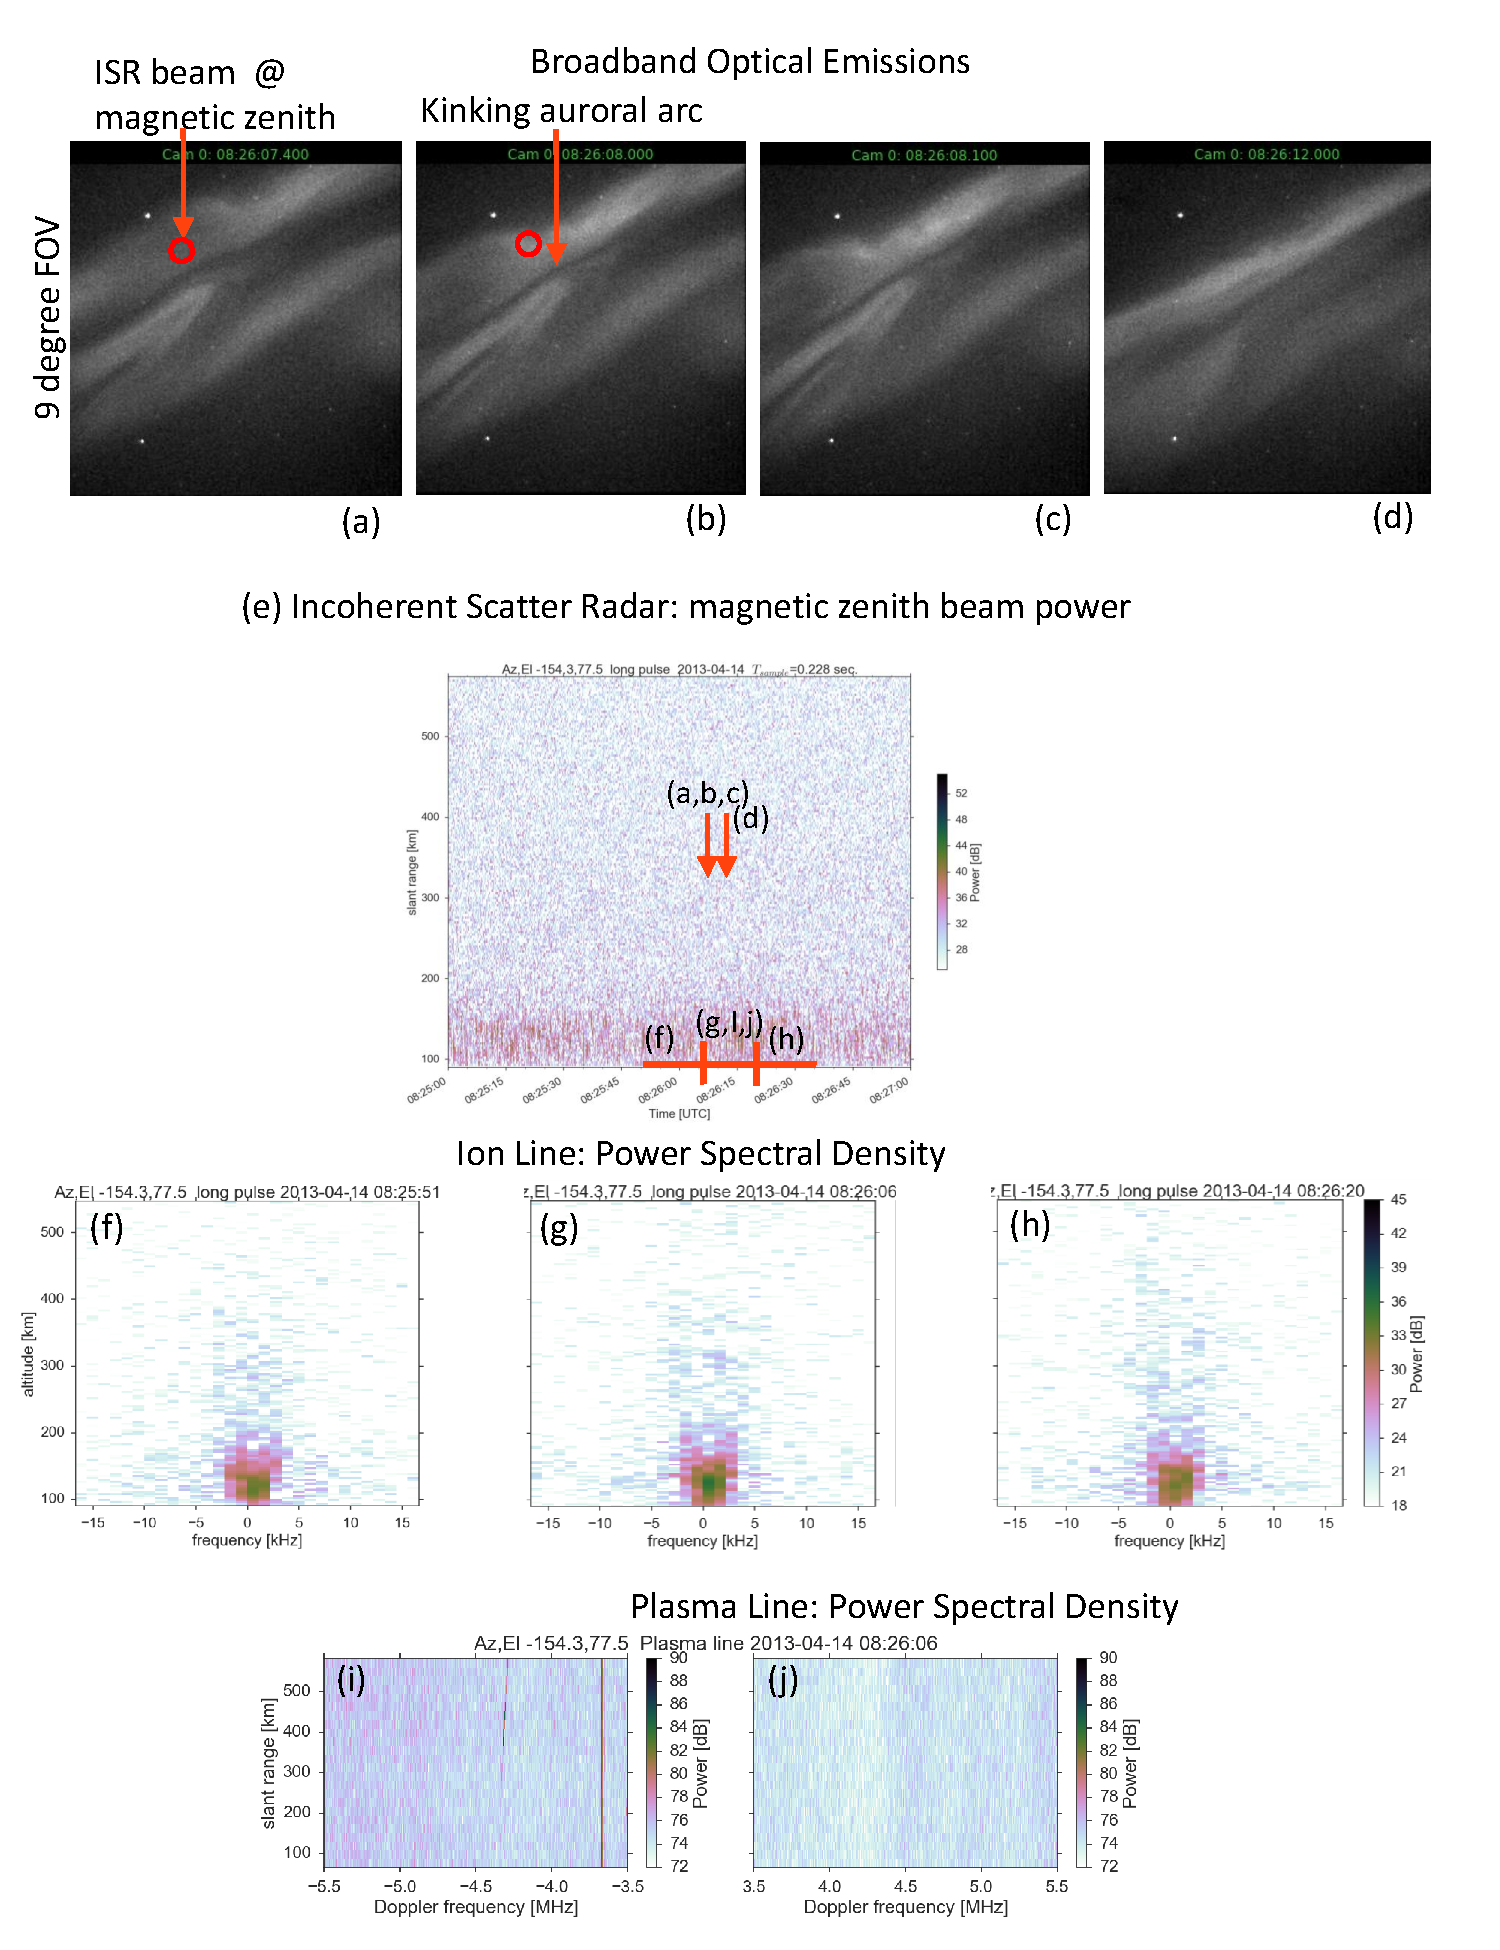
\includegraphics[width=\columnwidth,trim=15 697 25 0,clip]{gfx/2013-04-14T0826/2013-04-14T0826}

    \hspace{1.1cm}(a) 08:26:07.400 UT 
    \hspace{1.25cm}(b) 08:26:08.000 UT
    \hspace{1.1cm}(c) 08:26:08.100 UT
    \hspace{1.1cm}(d) 08:26:12.000 UT
    
    \caption{Narrow kinking and translating arcs at PFISR, ca. 08:26:10 UTC on April 14, 2013. 
          No coherent echoes detected in ion line, plasma line, or power spectral density.}
    %Two satellites cross through the field of view nearly orthogonally at 08:24:18 UTC.
    \label{fig:20130414T0826}
\end{sidewaysfigure}
A substorm is indicated as the initiator of the perturbation based on the southward turning IMF reflected in sharp negative excursion at 08:25 UTC as shown in Figure~\ref{fig:mag0826}.
\begin{figure}\centering
    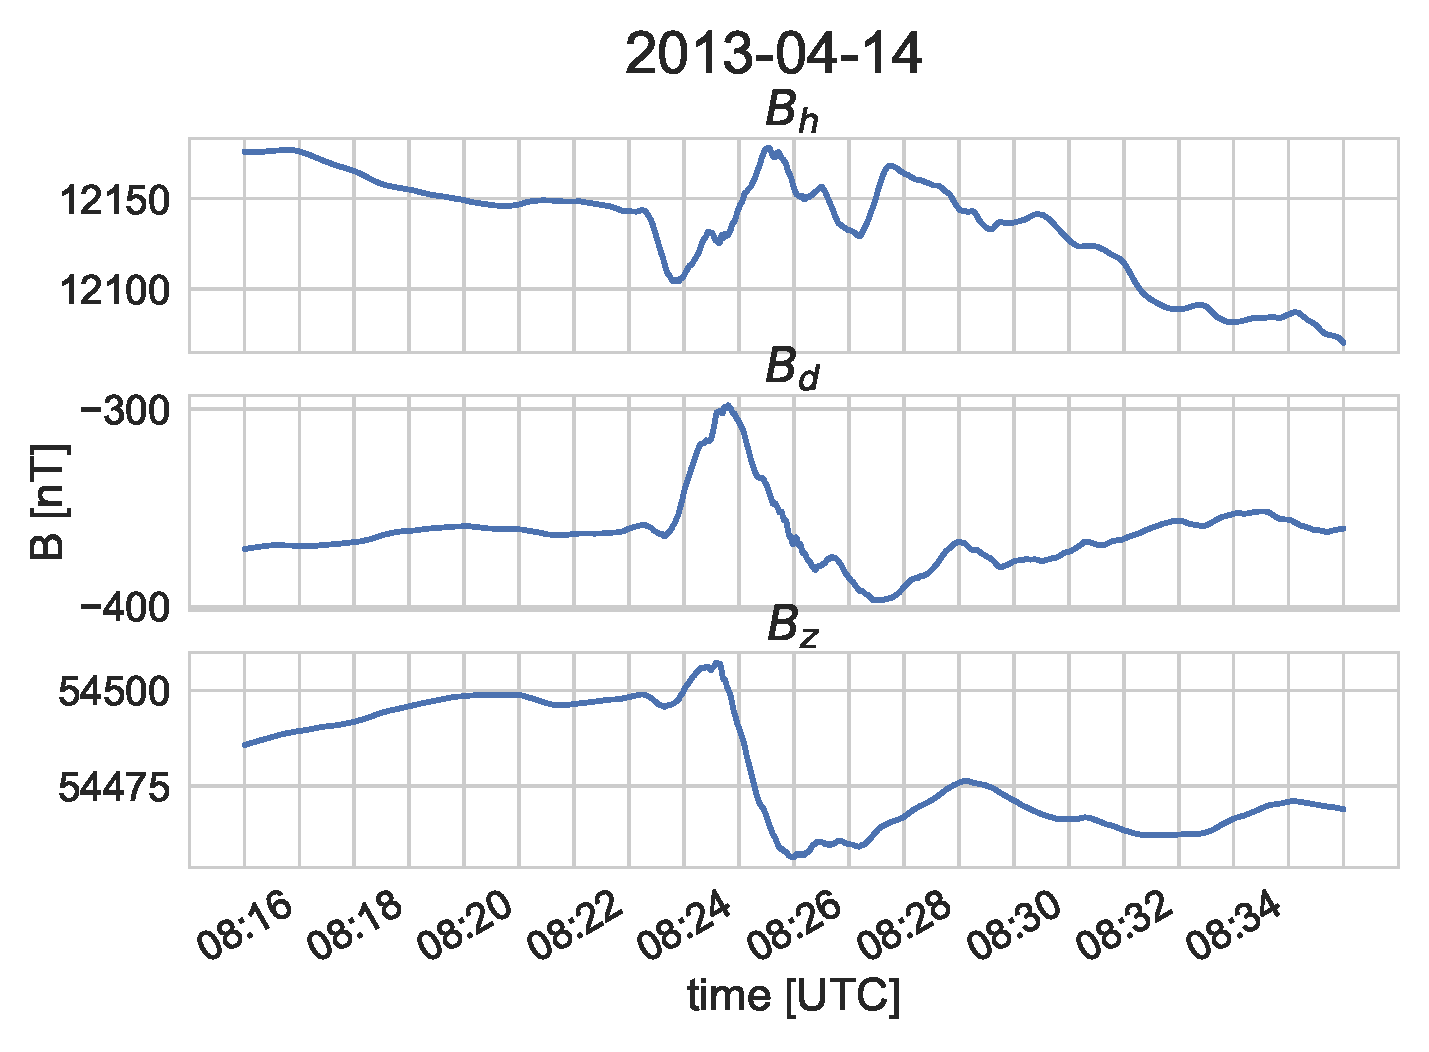
\includegraphics[width=\columnwidth]{gfx/2013-04-14T0826/mag}
    \caption{GIMA PFRR data showing geomagnetic field reversal near 08:25 UTC.}
    \label{fig:mag0826}
\end{figure}
A likely driver for this arc structure is an inverted-V acceleration region.
%As observed with HiST the auroral spectrum including the lines of Figure~\ref{fig:msp0826} is passed through the HiST BG3 filter, yielding $I_{557.7} \sim 0.01 \times I_{427.8}$.
The $I_{427.8}$ intensity suggests monoenergetic several keV electron beam configuration.
\begin{figure}
    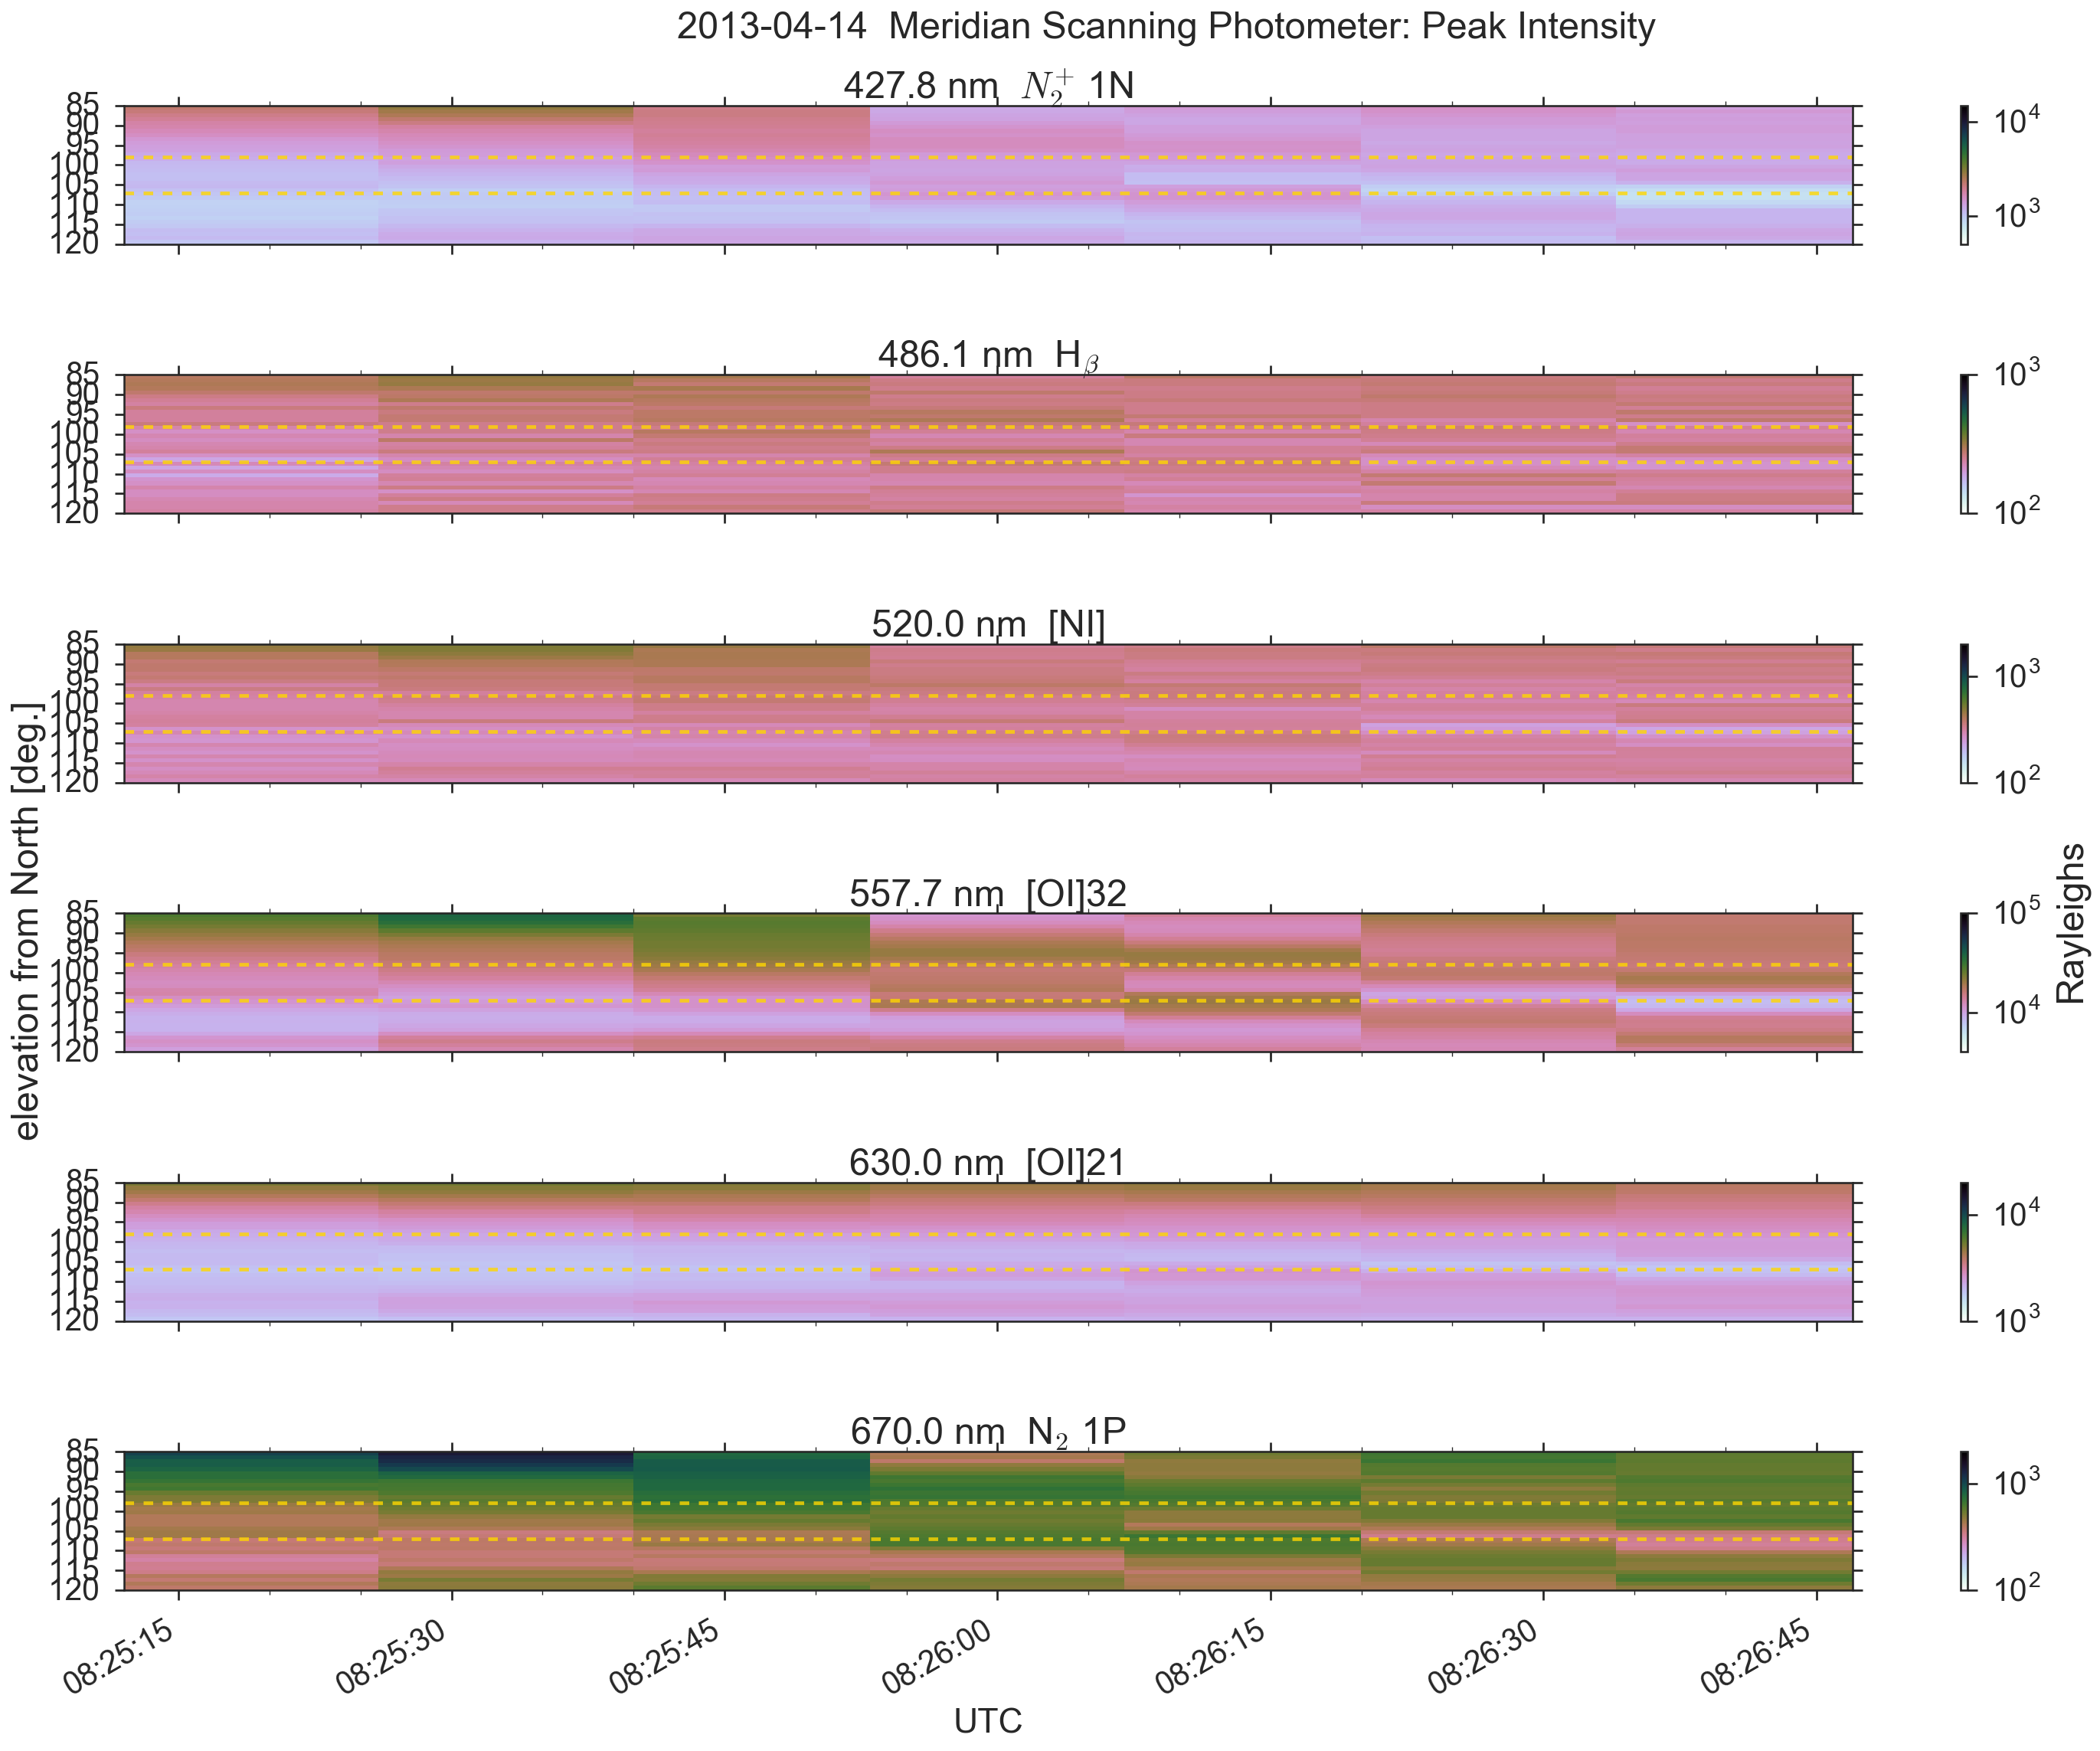
\includegraphics[width=\columnwidth]{gfx/2013-04-14T0826/msp_spectra}
    \caption{PF-DMSP spectrum showing strong $I_{427.8}$, suggesting monoenergetic beam of several keV driving kinked arc near 08:26 UTC.}\label{fig:msp0826}
\end{figure}
Monoenergetic inverted-V accelerated electron differential number flux in the several keV range is the most likely candidate for generating this kinked aurora.